\section*{Introduction}

\section{Data Extraction}

\section{Open source Datasets}

\section{Preprocessing}

\subsection{Artifact removal techniques}

\subsection{Spatial Filtering}

\subsection{Bipolar and Laplacian}

\subsection{Common Average Referencing}

\subsection{Independent Component Analysis}

\subsection{Common Spatial Patterns}

\subsection{Signal Space Projection}

\subsection{Feature Selection}

\subsection{Feature Extraction}

\subsection{Classification}

\section*{Summary}

% \section*{Introduction}
%     SLAM is analogous to Dynamic Bayes Network as shown in figure below. 
%     \begin{figure}[h] \label{fig:DBNOn}
%         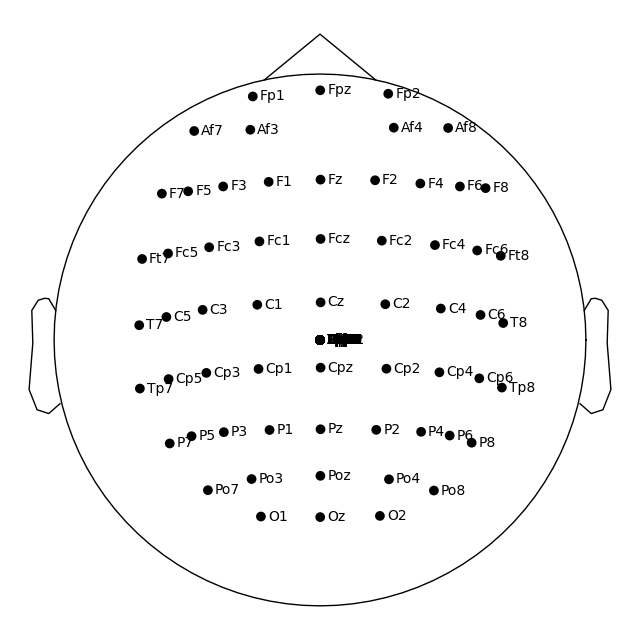
\includegraphics[width=0.9\textwidth]{images/BCI3IVa_Sensor_positions_(eeg).png}
%         \caption{Dynamic Bayes Network for Online SLAM. Source:\cite{Thrun98aprobabilistic}}
%     \end{figure}
%         The Pose information of the robot at time instant $t$ is represented as $x_t$ which constitutes $(x,y,\theta)$.
% where $(x,y)$ correspond to the location and $\theta$ represent orientation in the 2D Plane. Let $u_t$ be the Odometry reading of the motion executed between time $t-1$ and $t$. Let $Z_t$ be the LiDAR measurement taken at time $t$. Let $m$ be the Map created from the set of measurements. In figure \ref{fig:DBNOn}, the empty circles denote the states to be estimated and the shaded circles denote the variables that can be measured. Considering the circles to be the nodes and the arrows as edges, it is seen that the previous information on the state and the present command determines the current state of the system, which then influences the measurements obtained from map.The nodes $m$ and $x_{t+1}$ are the required output parameters. There are three basic fundamental approaches to the SLAM problem, namely, \textit{Kalman Filter}, \textit{Particle Filter}, \textit{Graph Network}. Each approach to the problem have their specific advantages and disadvantages, which will be discussed briefly in this chapter and extensively in upcoming chapters. However all the methods address the basic problem - Given the relative distance moved as recorded by the odometer and the observation at the current location, the system must be able to correctly localize and map its environment. In this chapter we will also look at how the probabilistic framework helps in achieving the task at hand and also the components commonly used across all the SLAM methods.
% %%%%%%%%%%%%%%%%%%%%%%%%%%%%%%%%%%%%%%%%%%%%%%%%%%%%%%%%%%%%%%%%%%%%%%%%%%%%%%%%%%%%%%%%%%%%%%%%%%%%%%%%%%%%%%
% \section{Probabilistic approach to state estimation}
%     In solving the \textit{online SLAM} Problem, the joint posterior distribution over the current pose and the map is the actual state of interest.
% \begin{equation} \label{eq:OnlSLM}
%     p(x_t, m | z_{1:t}, u_{0:t-1})
% \end{equation}
% whereas to solve the \textit{full SLAM }problem, the joint posterior distribution over  all the poses the robot had traversed and the map is the actual state of interest.
% \begin{equation} \label{eq:FullSLM}
%     p(x_{1:t}, m | z_{1:t}, u_{0:t-1})
% \end{equation}
% The distributions \ref{eq:FullSLM} and \ref{eq:OnlSLM} are applicable only to the grid based mapping because for Feature-based mapping the correspondence between the landmark measured and the measurement needs to be established and it is not estimated by the distributions mentioned above. This is a data association problem and it could be estimated as a part of the posterior distribution.
% \begin{equation} \label{CorresSLM}
%     p(x_{1:t}, m, c_t | z_{1:t}, u_{0:t-1})
% \end{equation}
% As this work is applicable only to grid-based mapping, Henceforth the derivations and equations are with respect to it without being mentioned explicitly.
% Applying the Bayes rule to determine the joint posterior distribution 
% \begin{equation} \label{eq:FullSLMc}
%     p(x_{1:t}, m | z_{1:t}, u_{0:t-1}) = \alpha . p(z_t | x_t, m).\int p(x_t| x_{t-1}, u_{t-1}). p(x_{1:t-1}, m | z_{1:t-1}, u_{0:t-2}) dx_{1:t-1}
% \end{equation}
% \par

% %EKF SLAM
% However estimating the states using \ref{eq:OnlSLM} becomes computationally expensive when integrating over all the previous poses and observation. This could be overcome by use of Extended KalmanFilter under three assumptions \textit{Feature-Based Maps} such that the number of landmarks are less , \textit{Gaussian Noise Assumption} such that the noise levels in the robot motion and perception is in limits that does not disturb the linearization of EKF and \textit{ Positive Information} such that unseen landmarks do not influence the estimation. In many practical applications the correspondence of a landmark to the measurement is not known. In such cases data association has to be derived during run time. In such cases, the correspondence is also estimated in the posterior distribution as shown in \refeq{eq:FullSLMc}.

% In the online SLAM process , as the robot moves through the environment, the system state vector and the covariance matrix are updated upon new measurements. 
% On observing new landmarks, new state variables are added to the system state vector and the covariance matrix. The EKF involves State Prediction and Correction step for every time a new information is received. The State Prediction and Correction steps are elaborated in subsequent sections. However the EKF has its own limitations. First, the covariance matrix maintained by the KalmanFilter has $K^2$ elements, where K is the number of landmarks. Hence the computational complexity rises to ${O}(K^2)$. Thus an increase in the number of the landmarks results in longer sensor updates. Second, The correspondence of the measurement and the landmarks is assumed to be known. Any wrong data association leads to filter divergence.  \par
% %RBPF SLAM
% Overcoming the problem, Rao-Blackwellized Particle Filters were used as a effective means to estimate the full posterior distribution. Instead of working on the entire distribution, particles were sampled at random and with sufficient number of particles the entire distribution could be covered.Here it is possible to relax the Gaussian assumption made in the EKF SLAM ,as any arbitrary distribution could be modelled as the target distribution. It basically involves steps such as Sampling, Importance Weighting, Re-sampling and Map Estimation. Sampling from proposal distribution corresponds to State prediction step and Importance Weighting corresponds to State Correction steps in EKF.
% More detailed discussion on RBPF is provided in the next chapter. This method is applicable to both Grid based and Feature Based mapping with fewer modifications.\par
% % %Graph SLAM
% % The third category of SLAM ...

% %%%%%%%%%%%%%%%%%%%%%%%%%%%%%%%%%%%%%%%%%%%%%%%%%%%%%%%%%%%%%%%%%%%%%%%%%%%%%%%%%%%%%%%%%%%%%%%%%%%%%%%%%%%%%%

% \section{State Prediction}
% State prediction is the key component in predicting the motion of the robot in case of EKF and Filter based SLAM methods, also it helps in creating the graph in front-end of graph based SLAM.The mobile robot is assumed to be equipped with odometer which provides relative motion of the wheels between time instances and a LiDAR sensor which can perceive the environment.Consider the positional state of the robot $x_{t-1}$ at time $t-1$, when subject to motion command $u_{t-1}$ the robot takes a new positional state $x_t$. The change in the positional state of the robot can be determined by use of motion models derived from translational and rotational kinematics or by using odometers. In equation \ref{eq:FullSLM}, the conditional density $p(x_t| x_{t-1}, u_{t-1})$ denote the state prediction part of the equation which could be replaced with appropriate motion models to predict the state of the robot in motion.The motion models derived will also need to factor the noise and uncertainty in its prediction, this is captured in the process noise covariance matrix. 

% \subsection{Odometry Motion Models}
% The odometers are basically wheel encoders which reads how much the wheels have moved through the environment on receiving the command. Hence it can only provide motion information post-the-fact, i.e. on receiving the motion command, the robot executes the command and then the odometry information is obtained. In many practical scenarios the robot might not follow all the motion commands as instructed due to slippage, wear and tear or due to any external forces. Under any such circumstances the odometer 
% provides much reliable information on the state of the robot. However 
% in case of motion planning this behaviour is not beneficial as the pose information at the next instance is critical to create a motion plan. In such cases the kinematic model of the 
% robot is used to predict the motion of the robot. 
% Algorithm for state prediction using odometry based motion model is very widely used in many robotics applications. Algorithms presented in the book \cite{Thrun98aprobabilistic} can be used off-the-self 
% for motion estimate implementation with odometry.
% On the downside, it is very common to observe drift and slippage in the odometer information and yet,it is most widely used in many robotics and industrial applications.

% \subsection{Kinematic Motion Models}
% In applications such as motion planning the positional state of the robot is required to be know in advance for planning and control. Depending on the number of tractions, dimensions of the robot the kinematic equations of the motion can be used to estimate the state of the system. \cite{R.Schubert} provides a detailed study on many different motion models which falls largely under the linear and curvilinear models. Linear motion models assume only straight motions and do not take rotations into account, whereas the curvilinear models assume the robot takes a circular path at a constant radius only exception being \textit{Constant Turn  Radius and Acceleration(CTRA)} which assumes that the robot follows a clothoid. The Figure \figurename{MtnMdl.png} provides the relationship and assumptions made by each of the motion models. \cite{R.Schubert}'s experiment results prove that curvilinear models provide better performance than linear models. Further CTRA shows better tracking results than the other curvilinear models. In \cite{Polack}, similar studies were made comparing Kinematic Bicycle Model and Dynamic models with 9-DOF, it was found that the earlier models were comparable to the dynamic model at low speeds and low angular acceleration. However at higher speeds or lateral
% acceleration ,the dynamic models with higher degrees of freedom were able to accurately plan the trajectory. Simplifying the solution to the problem and considering the theoretical  evidence in the literature, CTRA Motion Model is chosen as the motion model for state prediction in this thesis. The motion models derived are in continuous domain and these need to be discretized before it could be implemented on a computer. Methods such as Euler discretization or analytical methods are some of the common methods used in deriving discrete time representation of the process model and process covariance matrix. \cite{D.Svensson} provides the derivation of the discrete time equations for the CTRA model along with the process noise covariance modeled. The states involved in the prediction are longitudinal position ($x(t)$), lateral position ($y(t)$), heading angle ($\phi(t)$), speed ($s(t)$), acceleration ($a(t)$) and yaw rate ($\omega(t)$). In continuous domain the prediction function is derived and the discrete time model is derived using linearized discretization approach. The prediction equations are given by 
% \begin{gather} \label{CTRA_pred_ct}
%     x_{k+1}^{CTRA}
%     =
%     \begin{bmatrix} 
%         x_k \\ y_k \\ s_k \\ \phi_k \\ a_k\\ \omega_k
%     \end{bmatrix}
%     +
%     \begin{bmatrix} 
%         \Delta x_k \\ \Delta y_k \\ a_k T \\ \omega_k T \\ 0 \\ 0
%     \end{bmatrix}
%     + v_k
% \end{gather}
% where $T$ is predicition time and $v_k \thicksim  \mathcal{N}(0,Q_{k}^{CTRA})$ is the discrete time process noise that is a zero mean Gaussian noise with covariance $Q_k^{CTRA}$. For the complete derivation of the prediction function and the 
% process covariance matrix refer to \cite{D.Svensson}.

% %%%%%%%%%%%%%%%%%%%%%%%%%%%%%%%%%%%%%%%%%%%%%%%%%%%%%%%%%%%%%%%%%%%%%%%%%%%%%%%%%%%%%%%%%%%%%%%%%%%%%%%%%%%%%%
% \section{State Correction}
% The state of the system predicted using the motion models may not accurately define the state and its variance modeled using the process covariance matrix. In order to further deteremine 
% the exact posterior distribution, a confidence or a correction factor is required upon the predicted state. State correction techniques help in achieving a confidence or correction factor which helps in extracting precise information about the state predicted using the motion model. Various observation or measurement models can be chosen based on the sensor configuration present in the robot. In equation \ref{eq:FullSLM}, the conditional density $p(z_t | x_t, m)$ denotes the state correction part of the equation which can be replaced with appropriate measurement models or scan matching algorithms to estimate pose with confidence. Given the map $m$ and pose $x_t$ of the robot, the model must be able to summarise how the surrounding environment would seem to be. Numerous of research have been conducted on robot perception systems. Sensor systems such as LiDAR, Cameras, ultrasonic, radar are commonly used in various robotic applications depending on the environmental conditions where the robot is deployed.

% \subsection{Observation Models}
% In case of LiDAR, it is safe to asssume that every beam is independent of each other, hence the noise parameters and the measurement errors can be individually modelled. The measurement model density can thus be written as 
% \begin{equation}
%     p(z_t | x_t, m)  = \Pi_{k=1}^k  p(z_t^k | x_t, m)
% \end{equation}
% where  $z_t^k$ corresponds to a single laser beam. The density $p(z_t^k | x_t, m)$ can be modelled using different algorithms. Genrally it is a mixture of four distribution- Gaussian distribution at the incidence of an obstacle, exponentially decaying distribution to model unexpected objects in the view of actual obstacle, uniform distribution at the maximum range of laser beam and a uniform distribution throughout the range to include all unexpected measurements. The estimated value of the true measurement can be derived through ray casting operations in case of beam based models or nearest neighbour function in case of likelihood fields model\cite{Thrun98aprobabilistic}.  Algorithms suggested in the book \cite{Thrun98aprobabilistic} can be used off-the-shelf for estimating the ditribution.

% \subsection{Scan Matching}
% With advancement in computing power and use of LiDAR for perception it is possible to obtain more reliable results by registering two scans taken at two different relatively close poses and extract the relative poses between the two scans. This process of matching two scans is termed Scan Matching and it has been widely used for various applications. In other words, it is the method of finding the corrrect pose of the robot within a 3 dimensional search space which could provide the maximum value for the density $p(z_t | x_t, m)$. 
% \begin{equation}
%     \hat{x} _{t} = argmax_{x} p(x|m_{t-1}, z_t, x_t)
% \end{equation}
% \par
% Scan Matching is the core of this thesis. It will be discussed elaborately in subsequent chapters.

% \section{Summary}